\documentclass[twocolumn]{maeb2015}
\usepackage[latin1]{inputenc}
\usepackage[dvips]{epsfig}
\usepackage{graphicx}        % standard LaTeX graphics tool
\usepackage{subfigure}
\usepackage{url}

\def\BibTeX{{\rm B\kern-.05em{\sc i\kern-.025em b}\kern-.08em
    T\kern-.1667em\lower.7ex\hbox{E}\kern-.125emX}}


\begin{document}

\title{Aplicaci�n de T�cnicas de Inteligencia Computacional a Sistemas de Seguridad en la Empresa. \\El caso del proyecto MUSES} %!PN

% Primero: �Anna no participa? �Ni Sergio? Segundo �no hay nada mejor que sistemas de seguridad? �No ser�a, al menos, ciberseguridad? Sistemas de seguridad es para que no se metan los cacos - JJ

\author{P. De las Cuevas, A.M. Mora, J.J. Merelo \thanks{Departamento de Arquitectura y Tecnolog�a de Computadores. CITIC, ETSIIT,Universidad de Granada
E-mail: \{paloma,amorag,jmerelo\}@geneura.ugr.es}}

\maketitle

% �Qu� quieres hacer? �Cu�l es el objetivo? �Con qu� motivaci�n? �Qu�
% resultados nuevos o enfoque nuevo presentas en este trabajo? �Por
% qu� tendr�a que interesarle al lector? - JJ
\begin{abstract}
This paper presents an approach, based in a project in development, which combines Data Mining, Machine Learning and Computational Intelligence techniques, in order to create a user-centric and adaptable corporate security system. Thus, the system, named MUSES, will be able to analyse the user's behaviour (modelled as events) when interacting with the company's server, accessing to corporate assets, for instance. As a result of this analysis, and after the application of the aforementioned techniques, the Corporate Security Policies, and specifically, the Corporate Security Rules will be adapted to deal with new anomalous situations, or to better manage user's behaviour.
The work reviews the current state of the art in security issues
resolution by means of these kind of methods. Then it describes the
MUSES features in this respect and compares them with the existing
approaches.  
% ``en development'' suena a excusa y no aporta ninguna
% informaci�n. Igual que ha dicho Anna del cap�tulo de libro, lo que
% hay que presentar es el problema y la soluci�n, no el proyecto. El
% proyecto lo mencionas al final o en el estado del arte. - JJ
\end{abstract}

\begin{keywords}
Inteligencia Computacional, Inteligencia Artificial, Computaci�n Evolutiva, Algoritmos Evolutivos, Programaci�n Gen�tica, Seguridad Corporativa, Reglas de Seguridad
\end{keywords}

%-------------------------------------------------------------------
%%%%%%%%%%%%%%%%%%%%%%%% INTRODUCTION %%%%%%%%%%%%%%%%%%%%%%%%%%%%%%
%-------------------------------------------------------------------
\section{Introducci�n}
\noindent 

Security in distributed systems has been a very profitable research area from the arising of the first client/server architectures \cite{computer_security_80}. Inside this, corporate security is one of the main topics. The landscape has changed dramatically in the last years, starting with the distribution of the information (instead of being centralised in corporate servers, it has been spread among multiple machines such as portable devices, external servers, or cloud storage systems); and continuing with the so-called Bring Your Own Device (BYOD) philosophy, in which the devices that access to the system are owned by the users (company's employees), and could contain both personal and professional information.

This scenario opens up new security issues \cite{Opp_Security11}, which should be dealt in a different way, taking into account both (company's) data security and (user's) privacy. In order to protect them, there are defined \textit{Corporate Security Policies}.

To deal with this new situation, a novel system is being developed (inside an European Project). It is named \textit{MUSES}, from \textit{Multiplatform Usable Endpoint Security System} \cite{MUSES_SAC_14}, which is a device-independent end-to-end user-centric tool. 
It considers a set of security rules defined as specifications of the Company Security Policies, and its main feature is the ability of `learning' from the user's past behaviour and adapt, even inferring new ones, the set of rules in order to effectively manage potential future security incidents due to the user's behaviour. Then, the system will react, in a non-intrusive way, to the potentially dangerous sequence of actions (events) that he or she is conducting at any time.

To this end MUSES will analyse the users' behaviour by means of Data Mining
(DM) techniques \cite{DataMining_Lee01} and Machine Learning (ML) methods \cite{MachineLearning_Bishop06}, extracting a set of patterns which will be later processed by means of Computational Intelligence (CI) algorithms, mainly Evolutionary Computation methods \cite{EAs_Back96,GAs_Goldberg89,GP_Koza92}.

This is a step beyond the current state of the art in two senses: first regarding the current security systems for managing the new BYOD scenario inside the enterprises, as it can be read in \cite{MUSES_SAC_14}; and second concerning the application of Computational or Artificial Intelligence (AI) techniques to corporate security issues, focused on (and adapted to) the users' behaviour, as will be analysed in this work.

%Seguridad en la empresa, pol�ticas y reglas, computational intelligence en seguridad (breve).
%
%Cosas del DOW de por qu� es bueno aplicar cosas nuevas de CI a seguridad.
%Decir si hay algo hecho al respecto.

The paper is structured as follows. Next section gives a background in the current enterprise security issues. Section \ref{sec:stateofart} reviews related work regarding the application of DM, ML, AI and CI techniques to a wide range of security problems inside the enterprise, but mainly focused on the user's behaviour and the consequent security policies adaptation, which are the main advantages of MUSES.
The MUSES system's features regarding the application of those techniques are described in Section \ref{sec:muses_ci}. Then, these features are compared with the existing works reaching some conclusions in Section \ref{sec:conclusions}.


%-----------------------------------------------------------------
%%%%%%%%%%%%%%%%%%%%%%%% BACKGROUND %%%%%%%%%%%%%%%%%%%%%%%%%%%%%%
%-----------------------------------------------------------------
\section{Seguridad en la Empresa}

Until these days, enterprises used to follow a static Security Policy devoted to control a certain structure \cite{BYOD13}, where the Information Assets and the devices were purchased and maintained by the company. Now that corporate networks are becoming dynamic for being adapted to the BYOD philosophy, there is an additional risk because the devices that the employees use are not always company-owned. A needed security policy, or in this case, an \textit{Information Security Policy} (ISP from now on) should deal with the way of protecting a specific organisation information against a security breach. Though there are standards, such as the ISO27002 or the Security Forum's Standard of Good Practise\footnote{https://www.securityforum.org}, an ISP is defined depending on the characteristics of the community/organisation that they are built for.

Normally, the enterprise network architecture was being adapted to cope with external attackers \cite{MIT05}. However, with the consideration of BYOD, the threat is about corporate assets being compromised due to employees' devices with vulnerabilities \cite{android11}, or leaked because they are being accessed from a device connected through an unsecured (public) network.

%On the other hand, employee-owned devices, like smartphones, have the possibility of maintaining a good balance between work and private life. For this reason, the risk of uncontrolled devices (with potentially dangerous applications) accessing to corporate assets in unsafe conditions is bigger.

%Thus now, more things should be considered than the usual ones when designing a company network architecture. 
In Figure \ref{fig:proposed_diagram} there is a proposal which can be used for the beginning of the study of solutions that may make secure such a dynamic environment. It includes the possibility of having employee-owned mobile (smartphones and tablets) and portable (laptops) devices, and also the opportunity that the employees have of connecting these devices either from inside or outside the company premises. Moreover, company information assets are constantly accessed under these conditions, considering that an information asset means every \textit{piece of information} that has a \textit{value} (cost depending on the risk of being lost or leaked) for the company. It can be referred to files with sensitive information, to certain mails, or even to company applications.

\begin{figure}[ht]
	\begin{center}
		\includegraphics[scale=0.36]{proposed_diagram.eps}
		\caption{Architecture approach of an Enterprise Network assuming that the Company has adopted the BYOD philosophy.}
	\label{fig:proposed_diagram}
	\end{center}
\end{figure}

The other issue to cope with is the elaboration of a good ISP, understandable for all the users of the company, and more importantly, non-intrusive for them. A lot of researchers have studied the natural tendency of employees whether to comply or not with the ISP \cite{SecPolComp07,SecPolComp10,SecPolComp12}, reaching conclusions such as the employees compliance with the security policies increases educating/training them in information security awareness  \cite{SecPolComp09}, and decreases applying too much sanctions when a misuse or abuse occurs \cite{SecPolPenalty09}. 

This situation leads to a need of protecting the organisation side, but also the users side, making non-interfering easy-to-follow ISPs, and leaving them to use their devices for personal purposes while working, without putting corporate information assets under risk. The compliance of these requirements would compose an End-to-End Security Solution (protecting both enterprise and employee), which is the aim of the MUSES project \cite{MUSES_SAC_14} (see Section \ref{sec:muses_ci}).

%-----------------------------------------------------------------------
%%%%%%%%%%%%%%%%%%%%%%%% STATE OF THE ART %%%%%%%%%%%%%%%%%%%%%%%%%%%%%%
%-----------------------------------------------------------------------
\section{Estado del Arte}
\label{sec:soa}

Security is a wide area of research since the very beginning of the eighties \cite{computer_security_80}. Thousands of works have been published in a number of different issues in this topic. 
One of the most profiting fields is the application of Artificial Intelligence (AI) techniques to different security-based problems. This research line was started more than twenty years ago \cite{ai_intrusion_detection_94}, and will be still open for several years further \cite{ai_cybersecurity_11}.

The topics addressed by the researchers are quite varied, including Data Mining (DM) \cite{botnet_detection_clustering_09,feature_selection_anomalies_08}, and Machine Learning (ML) methods \cite{learning_network_intrusion_09,user_classification_ml_13}, applied to many different problems.

Computational intelligence techniques have been also widely used in this area, being the most profiting methods the Evolutionary Computation (EC) metaheuristics: Genetic Algorithms (GAs) and Genetic Programming (GP).

There are several works using GAs for solving security issues, such as the intrusion detection (see \cite{GA_intrusion_detection_survey_14} for a survey), the design and evaluation of security protocols \cite{detecting_intrusion_gp_03,eval_security_gas_07,GAs_security_protocols_10}, or the optimisation of different aspects related with security: IT security costs \cite{optimizing_IT_costs_ea_10} and cryptographic protocols \cite{cryptographic_gas_06}, to cite a few.

This work is focused on the application of different DM, ML and AI/CI techniques to a new set of security issues, which has arisen as a consequence of the new interactions between systems, and by the user's habits and behaviour (including the BYOD scenario), as it is described in Section \ref{sec:background}. 
Then, the works that we are interested in are those related with the users' information and behaviour (in this scope), and the management (and adaptation) of Information or Corporate Security Policies (ISPs).

In this line, the paper by Greenstadt and Beal \cite{cognitive_security_08} combined biometrics signals with ML methods in order to get a reliable user authentication in a computer system.
P.G. Kelley et al. \cite{user-controllable_learning_08} presented a method named \textit{user-controllable policy learning} in which the user gives feedback to the system every time that a security policy is applied, so these policies can be refined according to that feedback to be more accurate with respect to the user's needs. This approach could be useful for a personal device, but our aim in MUSES is to have a global set of rules that could be adapted for all the users.
On the other hand, policies could be created for enhancing user's privacy, as proposed by Danezis in \cite{inferring_policies_socialnetworks_09}, who defined a system able to infer privacy-related restrictions by means of a ML method applied in a social network environment. The idea of inferring policies will be also considered in MUSES, but in the scope of the company, and focused on ISPs.

A closer work to our approach is the one presented by Samak et al. \cite{policy_generation_clustering_10}, in which the authors use a clustering-based approach to infer new traffic security policies in a network.
However our idea in MUSES, explained in Section \ref{sec:muses_ci}, is to infer new Security Rules (as an specialisation of the ISPs) by means of GP.

Some other authors have applied this rule-based method for evolving (improving) a set of policies, such as Lim et al. \cite{sec_policy_evolution_gp_08,pol_evol_gp_3_approaches_08}, who inferred new policies based in the decisions on a system, considering the user's feedback. A similar approach will be considered in MUSES, but there will be an automatic evaluation system for the new inferred rules, rather to the strict need of a user control. Moreover, these works have been tested on synthetic testbeds, but MUSES will run in real companies with real users and real data.

Finally, the work by Suarez-Tangil et al. \cite{rule_generation_gp_09}, combines GP with the event correlation process which is also applied in MUSES \cite{MUSES_SAC_14}. However, their approach is designed to create the rules/engine for that process, instead of the security rules to be considered as the output of the event correlation, i.e. the decisions to be made according to the events produced and to the enterprise ISPs. 

The next section briefly presents the MUSES system, and describes the techniques to be used inside it, as mechanisms for ISPs adaptation to the user's behaviour.


%-------------------------------------------------------------
%%%%%%%%%%%%%%%%%%%%%%%% MUSEs %%%%%%%%%%%%%%%%%%%%%%%%%%%%%%
%-------------------------------------------------------------
\section{El Sistema MUSES}
\label{sec:muses}

As previously stated, MUSES will be a whole corporate security system aimed to deal with the new BYOD philosophy, i.e. it will manage user's accesses to the company servers from diverse own devices, which could be dangerous for several reasons, including the user's behaviour.

The defined MUSES architecture is shown in Figure \ref{fig:architecture_overview}.
%
\begin{figure*}[htp]
\centering
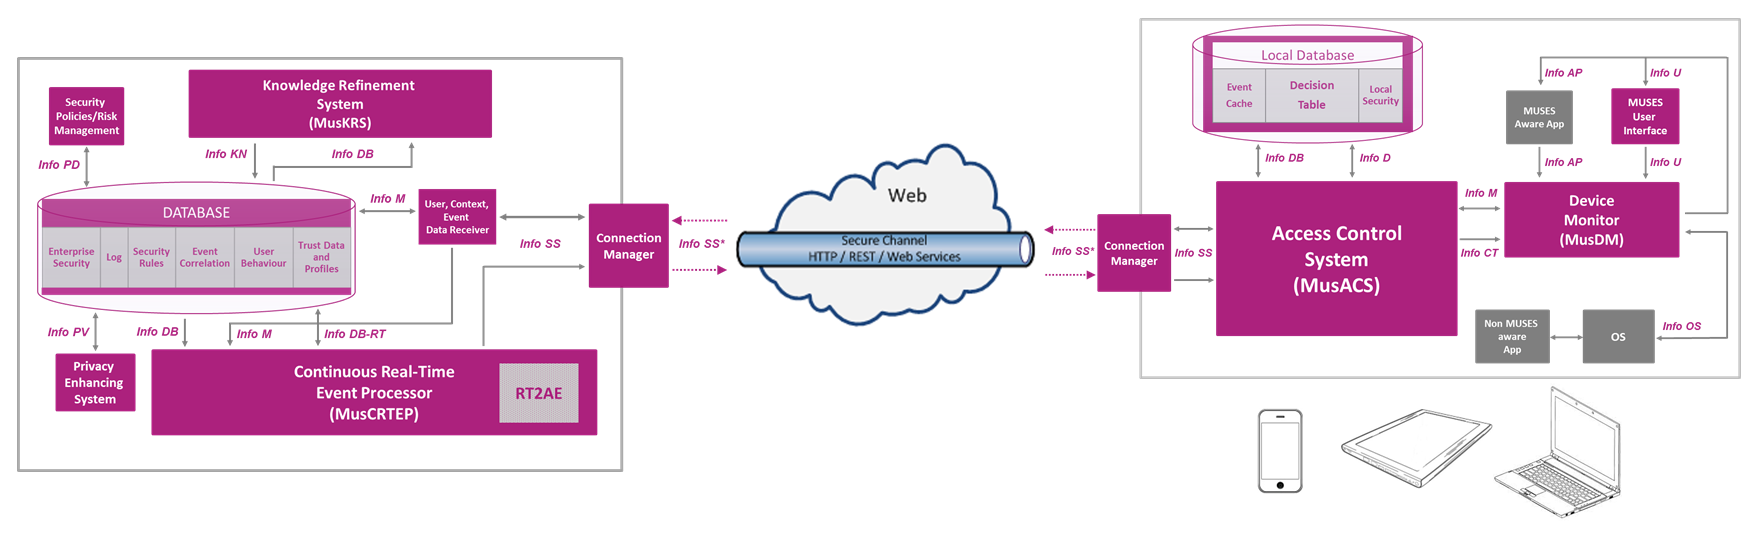
\epsfig{file=architecture_overview.eps, scale=0.61}
\caption{MUSES Architecture Overview (high-level components)\label{fig:architecture_overview}}
\end{figure*}
%
It is a \textit{client/server} approach in which the \textit{client} program will be installed in every user's mobile or portable device, independently of the platform (operating system and type of device). The \textit{server} side would be installed in the corporate security operations centre. Both sides are connected through a secure channel (using HTTPS) over Internet.

One of the main features of this system will be the self-adaptation (to the user and context) of the set of Corporate Security Rules (specification of the ISPs). 
To this end, there is a component in the designed architecture (Figure \ref{fig:architecture_overview}, left side) named \textit{MusKRS}, from MUSES \textit{Knowledge Refinement System}. This will be run asynchronously in the server and will be in charge of analysing all the gathered information (events, context, user-related data), and adapting/refining the security rules to better deal with these events, also trying to predict future threats due to the user's behaviour.

This process will be composed by two steps: first, a Data Mining/Machine Learning procedure will be performed (in the \textit{Data Miner} sub-component);  second, a refinement and inference process will be done (in the \textit{Knowledge Compiler} sub-component), considering the data `extracted' in the first step, by means of Computational Intelligence techniques.
It should be noticed that part of the refinement (or adaptation) of the security rules will be made using simpler methods, such as generalisation or specialisation of rules, for instance. Then, other parts of the process would be conducted using CI.

Another important fact is that MUSES will count with a human controller, normally the company Chief Security Officer (CSO), who will supervise the system activity by means of logs. Thus, adapted and inferred security rules will not be directly added to the current set of rules. Instead, they are proposed to this controller in order that he/she accepts them if they are interesting and correct. It is planned that the system will be able to `learn' from this decisions so, after a so-called training or `warm up' period, the rules would be directly accepted or rejected autonomously.

The following sections describe these processes: first focusing on DM techniques to be used both automatically by the KRS, and as a kind of decision-aid/monitoring tool for the CSO; second, the CI techniques are explained, mainly focusing in Evolutionary Computation approaches, since these methods perform very well, and have been widely used in security-based environments, as has been presented in Section \ref{sec:stateofart}.

% ------------------------------------------------------------------
%
\subsection{Data Mining/Machine Learning}
\label{subsec:dm_ml}

This task will be performed by the Data Miner module. It will take the `raw' data from the database and will process the information, in order to yield a set of relevant data for the Knowledge Compiler sub-component or for the human controller. In the first case, this sub-component will take them as a reference in order to refine or adapt the current set of security rules (for instance, to deal with anomalous situations).

The process will be mainly non-supervised, and eventually the datasets can be huge (depending on the company's data flows), so Big Data processing methods \cite{BigData_11} will be applied.

The DM/ML techniques will process the so-called patterns, which in this context correspond to events (and their related information) produced by the users' interactions with the system. The methods to be applied are:

\begin{itemize}

\item \textit{Pattern Mining} \cite{PatternMining_Han07}: 
This process will try to identify frequent or, on the contrary, anomalous patterns, in order to process them lately. The idea is that non-frequent patterns are potentially suspicious, and thus, could be of interest to be checked by the CSO or to serve as a reference for the rule-refinement process.

\item \textit{Classification} \cite{classification_67}: 
This technique tries to train a model (classifier) able to associate every pattern in the dataset to a class, so that the model could be used for assign a class for further incoming patterns with an unknown category.
For instance, it could look for events (patterns) that had been marked as `allowed' or `denied' (according to the ISPs). When a new event arises, if it has not an assigned decision, the classifier should provide one based on the similarity with previous (and already labelled) patterns.

\item \textit{Clustering} \cite{Clustering_Jain99}: 
The aim of this method is grouping the patterns considering some similarity criteria, in order to manage them as a set. This could be used for providing data visualisation mechanisms, in order to make it easier to interpret the data interaction and the distribution in clusters with respect to the different properties/features of the patterns.

\item \textit{Feature Selection} \cite{FeatureSelection_Guyon03}: 
It consists on extract the most important features/variables from the data. This could be useful if we want to discard non-key features, which could be interesting in order to reduce the database weight, for improving the performance of other techniques (such as classification or clustering), and even to improve the performance of whole the system, since less information would be gathered and transmitted.

\item \textit{Data Analysis}: 
This will provide the CSO with mechanisms to visualise interesting facts about the data, such as more frequent events, dangerous or suspicious users (according to their behaviour), more triggered rules, etc.

\end{itemize}

%\pagebreak

% ------------------------------------------------------------------
%
\subsection{Computational Intelligence: Evolutionary Computation Methods}
\label{subsec:ci}

%+ Clasificaci�n con GP
%- Inferencia de nuevas reglas con GP
%+ Ajuste de valores de recursos con AGs???

MUSES will use different EC approaches, initially, one in the DM/ML part of the process, and three in the rule-refinement/adaptation phase. They are based in GPs \cite{GP_Koza92}, and GAs \cite{GAs_Goldberg89}.

The first evolutionary-based approach will be a \textit{GP classification} method. This will be useful for two main reasons: first, in order to deal with the data class imbalance \cite{imbalance_techniques_02}, very common in classification problems inside real systems (with real data); and second, to better manage categorical (non-numeric) data, since most of the features/variables and information gathered from the events take these kind of values.

Thus, this approach will be able to manage unbalanced datasets considering a fitness function in which a cost can be associated to the classifier accuracy at every epoch, having a penalty cost when the classifier makes a false negative (an element from the minority class which is classified as belonging to the majority class) \cite{cost_adjustment_07}.
Regarding the type of data, since GP algorithms can manage rule- or tree-based models, it will work perfectly with any categorical variable, yielding a good classifier as it has been made in other works (such as the aforementioned \cite{cost_adjustment_07}).

The second set of EC approaches are, as stated, part of the rule-refinement (or adaptation) process. These techniques will be used for inference and optimisation, and will consider this data as a part of the process:

\begin{itemize}

\item The information extracted from the Data Miner sub-component, mainly concerning the anomalous, unclassified or misclassified patterns. These are those patterns which did not match with any of the existing classes (they are quite different from the patterns belonging to those classes), so they cannot be included in any of the classes and thus they should be taken into account for a potential inference or update in the set of security rules, in order to `cover' them.

\item User-related information corresponding to those anomalous or unlabelled patterns (events). Thus, the user's ID, location and role, for instance, will be considered in order to select the applicable set of rules for that conditions.

\item Context information for the same patterns, in order to also restrict the applicable set of rules considering this information. 

\end{itemize}

Another useful information to consider in the refinement/ adaptation process will be:

\begin{itemize}

\item Risk information extracted from the user profile (reputation), e.g. "Did the user received a lot of `denies'/`allows' before?", i.e. "Is he/she trustworthy?". In case the user is not, more restrictive rules would be created for him, otherwise the corresponding rules could be `eased' for that user.

\item The information stored in logs along the system, which can, for instance, tell about how the user responds to system messages (either an action or if he gives feedback). This could result in the inference of new rules or in adaptation, in order to deal with, for instance, users that repeatedly ignore warning messages.
Moreover, important log information regarding the parameters used or the decisions made in the different modules will be used for further tests of new inferred rules, as it is explained below.

\end{itemize}

So, the approaches that will be implemented are:

\begin{itemize}

\item \textit{GP rule inference} method, which will generate/create new rules in order to `cover' those situations non contemplated in the current set of rules. Thus, for instance, a new rule could be created in order to deal with the patterns to which the classifier could not assign a class.
The generation will be done considering the so-called \textit{dictionary}, i.e. a set of terms corresponding to all the possible inputs and actions in the system, which will be antecedents (conditions) and consequents in the security rules to be inferred.
The evaluation of these rules will be done considering the stored log information concerning the parameters along with the actions/decisions made in every component in the system. Thus, it will be possible to `simulate' the whole  system behaviour when the new rule is included and get a value of its performance.

\item \textit{GP rule refinement} approach, which will optimise the current set of rules, adjusting the values in the conditions (antecedents), for instance. Thus, some superfluous parts on the rules and even complete rules could be removed or improved, obtaining for instance specialisations or generalisations of existing rules which could mean a better performance.
The evaluation (of the whole set of security rules) will be done considering the number of unlabelled patterns that will be `covered' after the adjustments.

\item \textit{GA optimisation} algorithm for setting up and adapting the assets' values. These are numerical representations of the importance of the corporate assets, and are considered in the Real-Time Risk and Trust Analysis process, in order to assign a risk value to every potential decision that can be made by the system.
If it is possible to evaluate the partial solutions proposed by the GA, this approach could be very useful for the CSO (who is in charge of assigning and adjusting these values over time).
The adaptation or adjustment concerns the change in value that an asset could have due to a loss of importance, once an event has passed (a project presentation, for instance).

\end{itemize}


%-----------------------------------------------------------------
%%%%%%%%%%%%%%%%%%%%%%%% CONCLUSIONS %%%%%%%%%%%%%%%%%%%%%%%%%%%%%
%----------------------------------------------------------------- 
\section{Comparativa con Otros Sistemas y Conclusiones}
\label{sec:conclusion}

As it can be seen MUSES system will go quite far in the application of DM/ML techniques, with respect to other security-aimed systems. This was explained in the previous paper \cite{MUSES_SAC_14}, where the system was compared with other existing (commercial) systems.

Regarding the scientific contribution, one of the main differences with respect to previous works is the consideration of security threats `brought' by the user's behaviour inside the system, i.e. through interaction/events, rather than more general and external threats. Moreover, the techniques to be used here will work with real data (in a real system), as a difference to some research works.

Data Mining techniques have been used by the authors in some works, but usually aiming for a specific general objective, for instance the detection of threats (botnet) \cite{botnet_detection_clustering_09}, or the recognition of anomalies \cite{feature_selection_anomalies_08}, but they are not linked with a following process to improve the system (the refinement phase in MUSES).

There are some proposals in which security policies are inferred or refined \cite{inferring_policies_socialnetworks_09,policy_generation_clustering_10}, but they do not affect the ISPs as in MUSES, and they are not based in the user's behaviour in order to do this.

Genetic Programming has been previously used by several authors \cite{rule_generation_gp_09,sec_policy_evolution_gp_08}, even for creating new policies or rules in a security-aimed sense, but they do not affect the ISPs and moreover, our proposed evaluation functions (completely integrated in the system) for the refinement and inference approaches are novel.

With respect to Genetic Algorithms, they have been extensively used in the literature, mainly for the detection of anomalies and intrusions rather than for optimisation, as in our case. However, there are some examples that could be used as model for our approach, such as \cite{optimizing_IT_costs_ea_10,risk_reduction_ga_12}.

Anyway, there is room for considering some of the proposed approaches that could be added as future features for MUSES such as the analysis of users via social networks \cite{inferring_policies_socialnetworks_09,user_classification_ml_13}, the optimisation of security protocols \cite{GAs_security_protocols_10}, the implementation of intrusion detection mechanisms \cite{GA_intrusion_detection_survey_14}, or the application of novel privacy-related techniques \cite{AAI_book_2009}, which is another feature also considered in MUSES.

%******************************************************************************

\section*{Agradecimientos}
This work has been mainly supported by the MUSES European project (FP7-318508). In addition to PYR-2014-17 included in GENIL - CEI BIOTIC (Granada).

\nocite{*}
\bibliographystyle{maeb2015}

\begin{thebibliography}{1}

\bibitem{SecPolComp12}
A.~Al-Omari, O.~El-Gayar, A.~Deokar, and J.~Walters.
\newblock Security policy compliance: User acceptance perspective.
\newblock In {\em 45th Hawaii International Conference on System Sciences},
  pages 3317--3326. IEEE Press, 2012.

\bibitem{cost_adjustment_07}
E.~Alfaro-Cid, K.~Sharman, and A.~Esparcia-Alcázar.
\newblock A genetic programming approach for bankruptcy prediction using a
  highly unbalanced database.
\newblock In M.~Giacobini, editor, {\em Applications of Evolutionary
  Computing}, volume 4448 of {\em Lecture Notes in Computer Science}, pages
  169--178. Springer Berlin Heidelberg, 2007.

\bibitem{computer_security_80}
A.~J.~P. Anderson.
\newblock Computer security threat monitoring and surveillance.
\newblock Technical report, James P. Anderson Co., Fort Washington, PA, 1980.

\bibitem{BYOD13}
S.~Bacik.
\newblock {\em Information Security Management Handbook}, volume~7, chapter
  Security Implications of Bring Your Own Device, IT Consumerization, and
  Managing User Choices, pages 133--142.
\newblock Sixth edition, 2013.

\bibitem{EAs_Back96}
T.~Back.
\newblock {\em Evolutionary algorithms in theory and practice}.
\newblock Oxford University Press, 1996.

\bibitem{MachineLearning_Bishop06}
C.~Bishop.
\newblock {\em Pattern recognition and Machine Learning}.
\newblock Springer, 2006.

\bibitem{SecPolComp10}
B.~Bulgurcu, H.~Cavusoglu, and I.~Benbasat.
\newblock Information security policy compliance: an empirical study of
  rationality-based beliefs and information security awareness.
\newblock {\em MIS Quarterly}, 34(3):523--548, 2010.

\bibitem{botnet_detection_clustering_09}
S.~Chang and T.~E. Daniels.
\newblock P2p botnet detection using behavior clustering \& statistical tests.
\newblock In {\em Proceedings of the 2nd ACM Workshop on Security and
  Artificial Intelligence}, AISec '09, pages 23--30, New York, NY, USA, 2009.
  ACM.

\bibitem{inferring_policies_socialnetworks_09}
G.~Danezis.
\newblock Inferring privacy policies for social networking services.
\newblock In {\em Proceedings of the 2Nd ACM Workshop on Security and
  Artificial Intelligence}, AISec '09, pages 5--10, New York, NY, USA, 2009.
  ACM.

\bibitem{ai_intrusion_detection_94}
J.~Frank and N.~U. Mda-c.
\newblock Artificial intelligence and intrusion detection: Current and future
  directions.
\newblock In {\em In Proceedings of the 17th National Computer Security
  Conference}, 1994.

\bibitem{GAs_Goldberg89}
D.~E. Goldberg.
\newblock {\em Genetic Algorithms in search, optimization and machine
  learning}.
\newblock Addison Wesley, 1989.

\bibitem{learning_network_intrusion_09}
N.~G\"{o}rnitz, M.~Kloft, K.~Rieck, and U.~Brefeld.
\newblock Active learning for network intrusion detection.
\newblock In {\em Proceedings of the 2Nd ACM Workshop on Security and
  Artificial Intelligence}, AISec '09, pages 47--54, New York, NY, USA, 2009.
  ACM.

\bibitem{GA_intrusion_detection_survey_14}
P.~Gowher~Majeed and S.~Kumar.
\newblock Genetic algorithms in intrusion detection systems: A survey.
\newblock {\em International Journal of Innovation and Applied Studies},
  5(3):233--240, March 2014.

\bibitem{cognitive_security_08}
R.~Greenstadt and J.~Beal.
\newblock Cognitive security for personal devices.
\newblock In {\em Proceedings of the 1st ACM Workshop on Workshop on AISec},
  AISec '08, pages 27--30, New York, NY, USA, 2008. ACM.

\bibitem{FeatureSelection_Guyon03}
I.~Guyon and A.~Elisseeff.
\newblock An introduction to variable and feature selection.
\newblock {\em J. Mach. Learn. Res.}, 3:1157--1182, 2003.

\bibitem{PatternMining_Han07}
J.~Han, H.~Cheng, D.~Xin, and X.~Yan.
\newblock Frequent pattern mining: Current status and future directions.
\newblock {\em Data Min. Knowl. Discov.}, 15(1):55--86, 2007.

\bibitem{SecPolPenalty09}
T.~Herath and H.~Rao.
\newblock Protection motivation and deterrence: a framework for security policy
  compliance in organisations.
\newblock {\em European Journal of Information Systems}, 18:106--125, 2009.

\bibitem{Clustering_Jain99}
A.~K. Jain, M.~N. Murty, and P.~J. Flynn.
\newblock Data clustering: A review.
\newblock {\em ACM Comput. Surv.}, 31(3):264--323, Sept. 1999.

\bibitem{imbalance_techniques_02}
N.~Japkowicz and S.~Stephen.
\newblock The class imbalance problem: A systematic study.
\newblock {\em Intell. Data Anal.}, 6(5):429--449, Oct. 2002.

\bibitem{user-controllable_learning_08}
P.~G. Kelley, P.~Hankes~Drielsma, N.~Sadeh, and L.~F. Cranor.
\newblock User-controllable learning of security and privacy policies.
\newblock In {\em Proceedings of the 1st ACM Workshop on Workshop on AISec},
  AISec '08, pages 11--18, New York, NY, USA, 2008. ACM.

\bibitem{optimizing_IT_costs_ea_10}
T.~Kirta and J.~Kivimaab.
\newblock Optimizing it security costs by evolutionary algorithms.
\newblock In C.~Czosseck and K.~Podins, editors, {\em Conference on Cyber
  Conflict}, pages 145--160, Tallinn, Estonia, 2010. CCD COE Publications.

\bibitem{feature_selection_anomalies_08}
M.~Kloft, U.~Brefeld, P.~D\"{u}essel, C.~Gehl, and P.~Laskov.
\newblock Automatic feature selection for anomaly detection.
\newblock In {\em Proceedings of the 1st ACM Workshop on Workshop on AISec},
  AISec '08, pages 71--76, New York, NY, USA, 2008. ACM.

\bibitem{GP_Koza92}
J.~R. Koza.
\newblock {\em Genetic Programming: On the programming of computers by means of
  natural selection}.
\newblock MIT Press, Cambridge, MA, 1992.

\bibitem{DataMining_Lee01}
S.~J. Lee and K.~Siau.
\newblock A review of data mining techniques.
\newblock {\em Industrial Management \& Data Systems}, 101(1):41--46, 2001.

\bibitem{user_classification_ml_13}
A.~Leontjeva, M.~Goldszmidt, Y.~Xie, F.~Yu, and M.~Abadi.
\newblock Early security classification of skype users via machine learning.
\newblock In {\em Proceedings of the 2013 ACM Workshop on Artificial
  Intelligence and Security}, AISec '13, pages 35--44, New York, NY, USA, 2013.
  ACM.

\bibitem{pol_evol_gp_3_approaches_08}
Y.~T. Lim, P.~C. Cheng, J.~Clark, and P.~Rohatgi.
\newblock Policy evolution with genetic programming: A comparison of three
  approaches.
\newblock In {\em Evolutionary Computation, 2008. CEC 2008. (IEEE World
  Congress on Computational Intelligence). IEEE Congress on}, pages 1792--1800,
  June 2008.

\bibitem{sec_policy_evolution_gp_08}
Y.~T. Lim, P.~C. Cheng, P.~Rohatgi, and J.~A. Clark.
\newblock Mls security policy evolution with genetic programming.
\newblock In {\em Proceedings of the 10th Annual Conference on Genetic and
  Evolutionary Computation}, GECCO '08, pages 1571--1578, New York, NY, USA,
  2008. ACM.

\bibitem{MIT05}
R.~Lippmann, K.~Ingols, C.~Scott, K.~Piwowarski, K.~Kratkiewicz, M.~Artz, and
  R.~Cunningham.
\newblock Evaluating and strengthening enterprise network security using attack
  graphs.
\newblock Project report ia-2, Massachusetts Institute of Technology, Lincoln
  Laboratory, October 2005.

\bibitem{detecting_intrusion_gp_03}
W.~Lu and L.~Traore.
\newblock Detecting new forms of network intrusion using genetic programming.
\newblock In {\em Proceedings of the 2003 Congress on Evolutionary
  Computation}, pages 2165--2172, 2003.

\bibitem{classification_67}
J.~MacQueen et~al.
\newblock Some methods for classification and analysis of multivariate
  observations.
\newblock In {\em Proceedings of the fifth Berkeley symposium on mathematical
  statistics and probability}, volume~1, page~14. California, USA, 1967.

\bibitem{MUSES_SAC_14}
A.~Mora, P.~De~las Cuevas, J.~Merelo, S.~Zamarripa, M.~Juan,
  A.~Esparcia-Alc�zar, M.~Burvall, H.~Arfwedson, and Z.~Hodaie.
\newblock {MUSES: A corporate user-centric system which applies computational
  intelligence methods}.
\newblock In D.~S. et~al., editor, {\em 29th Symposium On Applied Computing},
  pages 1719--1723, 2014.

\bibitem{ai_cybersecurity_11}
B.~Morel.
\newblock Artificial intelligence and the future of cybersecurity.
\newblock In Y.~Chen, A.~A. C�rdenas, R.~Greenstadt, and B.~I.~P. Rubinstein,
  editors, {\em AISec}, pages 93--98. ACM, 2011.

\bibitem{Opp_Security11}
R.~Oppliger.
\newblock Security and privacy in an online world.
\newblock {\em IEEE Computer}, 44(9):21--22, September 2011.

\bibitem{android11}
C.~Orthacker, P.~Teufl, S.~Kraxberger, G.~Lackner, M.~Gissing, A.~Marsalek,
  J.~Leibetseder, and O.~Prevenhueber.
\newblock Android security permissions - can we trust them?
\newblock In {\em MobiSec Session on Smartphone Security}, Aalborg, 2011.

\bibitem{BigData_11}
B.~Ratner.
\newblock {\em Statistical and Machine-Learning Data Mining: Techniques for
  Better Predictive Modeling and Analysis of Big Data, Second Edition}.
\newblock CRC Press, Inc., Boca Raton, FL, USA, 2nd edition, 2011.

\bibitem{policy_generation_clustering_10}
T.~Samak and E.~Al-Shaer.
\newblock Synthetic security policy generation via network traffic clustering.
\newblock In {\em Proceedings of the 3rd ACM Workshop on Artificial
  Intelligence and Security}, AISec '10, pages 45--53, New York, NY, USA, 2010.
  ACM.

\bibitem{SecPolComp09}
R.~Shaw, C.~Chen, A.~Harris, and H.-J. Huang.
\newblock The impact of information richness on information security awareness
  training effectiveness.
\newblock {\em Computers \& Education}, 52:92--100, 2009.

\bibitem{SecPolComp07}
M.~Siponen, S.~Pahnila, and A.~Mahmood.
\newblock {\em {New Approaches for Security, Privacy and Trust in Complex
  Environments}}, volume 232, chapter {Employees' adherence to information
  security policies: an empirical study}, pages 133--144.
\newblock IFIP International Federation for Information Processing, 2007.

\bibitem{AAI_book_2009}
A.~Solanas and A.~Mart�nez-bal.
\newblock {\em Advances in Artificial Intelligence for Privacy Protection and
  Security}.
\newblock World Scientific Publishing Co., Inc., River Edge, NJ, USA, 2009.

\bibitem{rule_generation_gp_09}
G.~Suarez-Tangil, E.~Palomar, J.~Fuentes, J.~Blasco, and A.~Ribagorda.
\newblock Automatic rule generation based on genetic programming for event
  correlation.
\newblock In l.~Herrero, P.~Gastaldo, R.~Zunino, and E.~Corchado, editors, {\em
  Computational Intelligence in Security for Information Systems}, volume~63 of
  {\em Advances in Intelligent and Soft Computing}, pages 127--134. Springer
  Berlin Heidelberg, 2009.

\bibitem{risk_reduction_ga_12}
A.~Tamjidyamcholo.
\newblock Genetic algorithm approach for risk reduction of information
  security.
\newblock {\em International Journal of Cyber-Security and Digital Forensics
  (IJCSDF)}, 1(1), 2012.

\bibitem{GAs_security_protocols_10}
L.~Zarza, J.~Forn�~Mu�oz, J.~R. Pegueroles~Vall�s, and M.~Soriano~Ib��ez.
\newblock {\em Advances in artificial intelligence for privacy protection and
  security}, chapter Genetic algorithms for designing network security
  protocols, pages 325--358.
\newblock World Scientific, 2010.

\bibitem{eval_security_gas_07}
L.~Zarza, J.~Pegueroles, and M.~Soriano.
\newblock Evaluation function for synthesizing security protocols by means of
  genetic algorithms.
\newblock In {\em Proceedings of the The Second International Conference on
  Availability, Reliability and Security}, ARES '07, pages 1207--1213,
  Washington, DC, USA, 2007. IEEE Computer Society.

\bibitem{cryptographic_gas_06}
L.~Zarza, J.~Pegueroles, M.~Soriano, and R.~Mart�nez.
\newblock Design of cryptographic protocols by means of genetic algorithms
  techniques.
\newblock In M.~Malek, E.~Fern�ndez-Medina, and J.~Hernando, editors, {\em
  SECRYPT}, pages 316--319. INSTICC Press, 2006.

\end{thebibliography}
\end{document}
